\chapter{振子、占据数与第一个量子场}

量子场论是我们处理几乎所有已知非引力物理的框架。这一说法不应与“每个问题都能被解决”的说法相混淆。氢原子尚可处理；到了诸如硼这样的原子，计算就已经困难得多，而一个人则远远超出任何现实的场论计算能力。这个框架也许是基本的，但它的方程仍然极其困难。

因此我们将以尽可能初等的方式进入。这个主题有时被称为\emph{二次量子化}，但在我们建立起这套机器之前，这个名字意义不大。最短的路径不是从相对论性场开始，而是从谐振子开始。弹簧并不是重点。重要的是升算符与降算符的代数。一旦这套代数对许多模式重复，升算符将不再仅仅意味着``把一个振子提升一个能级''，而将字面地意味着``产生一个粒子。''

\section{作为代数的振子}

对于一个振子，令\(a^\dagger\)提升激发，令\(a\)降低它。记号\(a_+\)与\(a_-\)是等价的，但匕首记号预示了场论中使用的语言。最低态满足
\begin{equation}
a|0\rangle=0,
\end{equation}
而数算符为
\begin{equation}
N=a^\dagger a,
\qquad
N|n\rangle=n|n\rangle.
\end{equation}
这两个阶梯算符互为厄米共轭，它们本质的对易子是
\begin{equation}
[a,a^\dagger]=1.
\label{eq:l06-single-commutator}
\end{equation}
这个小代数几乎就是整个振子。

人们可以从位置与动量的适当线性组合中恢复出\(a\)与\(a^\dagger\)。具体约定取决于\(x\)、\(p\)、\(m\)与\(\omega\)的归一化；这里有用的不变陈述是，\(a^\dagger a\)除了其相加的基态能量之外，重构了二次型振子哈密顿量。因此
\begin{equation}
H=\hbar\omega\left(N+\frac12\right).
\end{equation}
在目前的讨论中，我们丢掉常数项并使用
\begin{equation}
H=\hbar\omega N.
\label{eq:l06-one-oscillator-hamiltonian}
\end{equation}
频率告诉我们一个激发的代价。把\(n\)提升一需要\(\hbar\omega\)；把\(n\)降低一释放同样的量。

\section{许多独立振子}

现在取许多振子并用\(i\)标记它们。这个标记只是一个指标，不是虚数单位。模式可以有有限多个，也可以有无限多个。一组独立弹簧给出一种图像；理想小提琴弦的简正模式给出另一种。在场论应用中，无限集合是重要的情形。

独立性有一种算符含义。属于真正独立子系统的算符对易。如果它们不对易，相应的量就不能被独立测量，而这些系统从一开始就不是独立的。因此我们有
\begin{align}
[a_i,a_j]&=0, \\
[a_i^\dagger,a_j^\dagger]&=0, \\
[a_i,a_j^\dagger]&=\delta_{ij}.
\label{eq:l06-many-commutators}
\end{align}
对于\(i\ne j\)，属于这两个模式的一切都对易。对于\(i=j\)，最后一行化为式~\eqref{eq:l06-single-commutator}。

每个振子都有自己的数算符，通常也有自己的频率：
\begin{equation}
N_i=a_i^\dagger a_i,
\qquad
H=\sum_i\hbar\omega_i N_i.
\label{eq:l06-many-hamiltonian}
\end{equation}
共同本征态由下面这组完整的数标记：
\begin{equation}
|n_1,n_2,n_3,\ldots\rangle,
\qquad n_i=0,1,2,\ldots.
\label{eq:l06-occupation-ket}
\end{equation}
整数\(n_i\)称为第\(i\)个振子的\emph{占据数}。在这个阶段，这还只是一个术语。很快，它就会用来计数占据某个单粒子态的粒子数，这个名称也就有了字面上的含义。

所有占据数都等于零的态是
\begin{equation}
|0\rangle\equiv|0,0,0,\ldots\rangle,
\qquad a_i|0\rangle=0\quad\text{for every }i.
\label{eq:l06-oscillator-vacuum}
\end{equation}

\begin{classroomqa}
\lecturetimestamp{00:15:27}
\audiencequestion{无限多个振子的族是否对应于诸如小提琴弦这样的系统的连续模式？}
\lecturerresponse{是的，在理想化弦中如此。真实的弦由原子构成，因此足够短的波长最终会遇到微观截断。尽管如此，连续模型为场论中使用的无限多个模式提供了动机。}
\end{classroomqa}

\section{为什么阶梯系数是平方根}

\(a^\dagger\)的作用必须把\(N\)的一个本征态提升到下一个本征态，但归一化留下了一个系数的余地：
\begin{equation}
a^\dagger|n\rangle=c_n|n+1\rangle.
\label{eq:l06-unknown-coefficient}
\end{equation}

\begin{figure}[htbp]
\centering
\includegraphics[width=0.9\linewidth]{lecture_06_frame_01.png}
\caption{阶梯系数是在其归一化被推导出来之前引入的。黑板上的方程在式~\eqref{eq:l06-unknown-coefficient}中重现。}
\lectureframe{00:19:38}
\end{figure}

选择使\(c_n\)为实的相位约定。取厄米共轭给出
\begin{equation}
\langle n|a=c_n\langle n+1|.
\end{equation}
将这两个关系相乘并使用归一化基态，
\begin{align}
c_n^2
&=\langle n|aa^\dagger|n\rangle \\
&=\langle n|(a^\dagger a+1)|n\rangle \\
&=\langle n|(N+1)|n\rangle \\
&=n+1.
\end{align}
因此，
\begin{equation}
a^\dagger|n\rangle=\sqrt{n+1}\,|n+1\rangle.
\label{eq:l06-raising-rule}
\end{equation}

\begin{classroomqa}
\lecturetimestamp{00:22:35}
\audiencequestion{为什么可以在求出\(c_n\)之前先设定\(\langle n+1|n+1\rangle=1\)？}
\lecturerresponse{本征矢量从一开始就被选为归一化基。它们的归一化并不决定\(a^\dagger|n\rangle\)的归一化；那剩余的信息恰恰就是系数\(c_n\)。}
\end{classroomqa}

下降规则以同样的方式得到：
\begin{equation}
a|n\rangle=\sqrt n\,|n-1\rangle.
\label{eq:l06-lowering-rule}
\end{equation}
在\(n=0\)处，系数自动为零，因此该规则包含\(a|0\rangle=0\)。对于多个模式，该算符只改变其自身位置上的占据数：
\begin{align}
a_i^\dagger|n_1,\ldots,n_i,\ldots\rangle
&=\sqrt{n_i+1}\,|n_1,\ldots,n_i+1,\ldots\rangle, \\
a_i|n_1,\ldots,n_i,\ldots\rangle
&=\sqrt{n_i}\,|n_1,\ldots,n_i-1,\ldots\rangle.
\label{eq:l06-multimode-ladders}
\end{align}
其他条目不受影响。

\section{波函数不是量子场}

在定义场之前，我们必须把它与熟悉的波函数区分开来。三组对比组织了这一过渡。

第一，单粒子波函数
\begin{equation}
\psi(x)=\langle x|\psi\rangle
\end{equation}
是态矢量的一个表示。它本身不是可观测量。我们测量位置、动量、角动量以及其他算符；波函数提供振幅，由这些振幅计算出那些结果的概率。

第二，多粒子波函数依赖于所有粒子的位置。对于两个粒子，其位置矢量暂时称为\(x\)和\(y\)，
\begin{equation}
\psi(x,y)=\langle x,y|\psi\rangle.
\end{equation}
这里\(x\)和\(y\)标记两个不同的粒子；它们不是一个位置矢量的两个笛卡儿\(x\)分量和\(y\)分量。对于\(N\)个粒子，态由下式表示
\begin{equation}
\psi(x_1,x_2,\ldots,x_N).
\end{equation}

第三，这个波函数描述固定数目的粒子。一个十五粒子波函数有十五个位置自变量，属于十五粒子希尔伯特空间。它本身并不描述粒子数从十五变为十四或十六的过程。

量子场将反转这些特征。它是算符而不是态，它依赖于一个空间点\(x\)，并且作用在一个包含每个粒子数扇区的态空间上。短语``一个点''意味着一个可自由变化的位置矢量。它并不意味着\(x\)已被赋予一个数值。

有一个限定条件在以后会很重要。下面引入的场\(\Psi(x)\)不是厄米的，因此它本身在严格意义上不是可观测量。它的厄米组合才是可观测量。因此，场是可测量的这一临时说法被精确化，而不是被抛弃：场是算符值函数，而它们的厄米组合表示可测量的量。

\begin{classroomqa}
\lecturetimestamp{00:36:52}
\audiencequestion{如果场是一个位置的函数，那个位置可以变化吗？还有，双粒子波函数中的\(y\)到哪里去了？}
\lecturerresponse{点\(x\)在整个空间中变化。``一个位置''意味着该算符有一个空间自变量，而不是说该自变量是固定的。在\(\psi(x,y)\)中，符号\(x\)和\(y\)命名两个粒子的位置；等价地，它们是\(x_1\)和\(x_2\)。它们不是场自变量的两个笛卡儿分量。}
\end{classroomqa}

\begin{classroomqa}
\lecturetimestamp{00:38:15}
\audiencequestion{固定粒子波函数描述和场描述如何关联，它们描述的是不同种类的粒子吗？}
\lecturerresponse{这一联系就是仍将给出的核心构造。粒子是同一种类的。在本讲中它们是玻色子；费米子需要不同的代数。}
\end{classroomqa}

\section{盒中单粒子}

暂时回到普通的单粒子量子力学。把一个粒子放入一维盒中。只有一个粒子时，玻色子和费米子之间的区别无关紧要：没有第二个全同粒子可以用来检验交换或排除。

令
\begin{equation}
\psi_1(x),\ \psi_2(x),\ \psi_3(x),\ldots
\end{equation}
为能量本征函数。最低模式是在壁处消失的最平滑的波。下一个模式有一个内部节点，而更高能量的模式振荡得更快。在宽度为\(L\)的理想无限深方势阱中，一个方便的归一化基是
\begin{equation}
\psi_i(x)=\sqrt{\frac{2}{L}}\sin\!\left(\frac{i\pi x}{L}\right),
\qquad 0<x<L.
\label{eq:l06-box-basis}
\end{equation}
显式的正弦公式是定性黑板草图的一个标准实现；下面的论证只需要一组完备正交归一的单粒子态。

\begin{figure}[htbp]
\centering
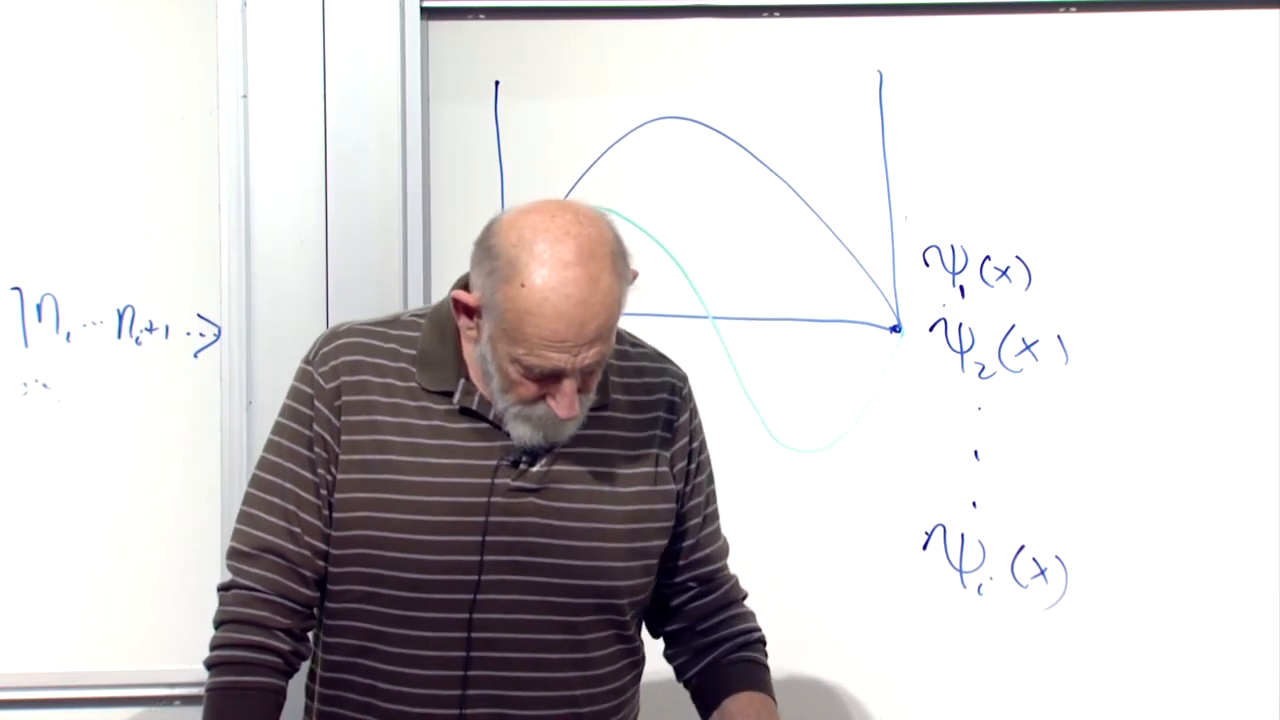
\includegraphics[width=0.9\linewidth]{lecture_06_frame_03.png}
\caption{按能量递增排列的单粒子盒模式。第一个模式没有内部节点，第二个有一个，省略的更高模式振荡得越来越快。}
\lectureframe{00:43:10}
\end{figure}

同样的结构可以在没有现场黑板遮挡的情况下重新绘制：
\begin{figure}[htbp]
\centering
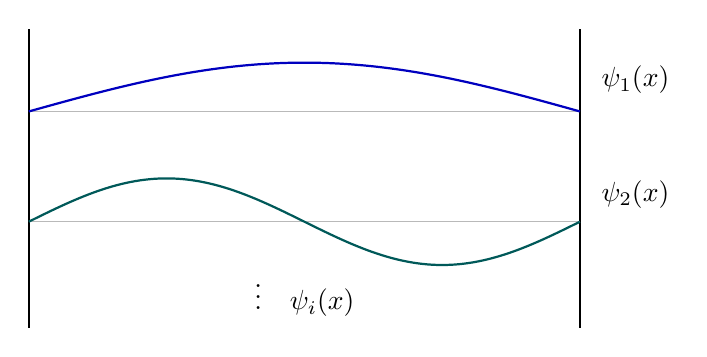
\begin{tikzpicture}[x=1cm,y=1cm]
  \draw[thick] (0,0) -- (0,3.8);
  \draw[thick] (7,0) -- (7,3.8);
  \draw[gray!55] (0,2.75) -- (7,2.75);
  \draw[gray!55] (0,1.35) -- (7,1.35);
  \draw[blue!75!black,thick,domain=0:7,samples=120]
    plot (\x,{2.75+0.62*sin(180*\x/7)});
  \draw[teal!70!black,thick,domain=0:7,samples=120]
    plot (\x,{1.35+0.55*sin(360*\x/7)});
  \node[right] at (7.15,3.15) {$\psi_1(x)$};
  \node[right] at (7.15,1.70) {$\psi_2(x)$};
  \node at (3.5,0.45) {$\vdots\quad \psi_i(x)$};
\end{tikzpicture}
\caption{定性盒模式草图的清晰重建。垂直位移是为了可读性而将本征函数分开，并不是额外的物理坐标。}
\end{figure}

指标\(i\)标记的是一个单粒子态，而不是一个粒子，也不是节点数。对于盒基，\(i\)恰好比内部节点数多一。每个态都有一个能量\(\varepsilon_i\)。按照讲座的记号，我们可以把这个能量写成\(\hbar\omega_i\)，或者在令\(\hbar=1\)之后简单地写成\(\omega_i\)。

\begin{classroomqa}
\lecturetimestamp{00:39:01}
\audiencequestion{先前的独立性假设是精确的吗，指标\(i\)能否标记原子中电子的可能状态？}
\lecturerresponse{对于独立模式构造，不同模式之间的对易是精确的。该指标可以标记单粒子原子态。然而，如果粒子之间存在相互作用，简单的独立模式哈密顿量就不再是全部内容了。}
\end{classroomqa}

\begin{classroomqa}
\lecturetimestamp{00:40:34}
\audiencequestion{盒中的粒子是玻色子吗？}
\lecturerresponse{它可能是，但只有一个粒子时，统计性质无关紧要。只有当存在多于一个全同粒子时，排斥和交换才有意义。}
\end{classroomqa}

\section{从盒模式到福克空间}

现在允许盒中有任意数量的全同玻色子。某个数目\(n_1\)可以占据\(\psi_1\)，某个数目\(n_2\)可以占据\(\psi_2\)，依此类推。因此一个基态是
\begin{equation}
|n_1,n_2,n_3,\ldots\rangle.
\end{equation}
这正是已经用于多振子的记号。这种等同是结构性的：把每一个单粒子态与一个振子联系起来，并把振子激发数等同于占据该态的粒子数。

玻色子在这里是本质性的，因为每个\(n_i\)都可以是任意非负整数。对于费米子，每个单粒子态可以是空的或单占据的，绝不能双占据，因此普通的振子代数不能原封不动地使用。

现在可以通过算符对占据数基的作用来定义它们。算符\(a_i^\dagger\)在单粒子态\(i\)中产生一个粒子；\(a_i\)移除一个：
\begin{align}
a_i^\dagger|n_1,\ldots,n_i,\ldots\rangle
&=\sqrt{n_i+1}\,|n_1,\ldots,n_i+1,\ldots\rangle, \\
a_i|n_1,\ldots,n_i,\ldots\rangle
&=\sqrt{n_i}\,|n_1,\ldots,n_i-1,\ldots\rangle.
\end{align}
这并非事后类比。这就是玻色子产生和湮灭算符在这个基上的定义。因为该基张成整个空间，所以这个定义通过线性性决定了它们对每一个态的作用。

\begin{classroomqa}
\lecturetimestamp{00:47:11}
\audiencequestion{\(n_1,n_2,n_3\)是量子态吗？}
\lecturerresponse{标签\(1,2,3,\ldots\)标识单粒子态。符号\(n_1,n_2,n_3,\ldots\)是占据这些态的粒子数。把态标签与其占据数保持区分是主要的记号负担。}
\end{classroomqa}

\subsection{平方根起什么作用}

因子\(\sqrt{n_i+1}\)并不表示一个额外的粒子或一个单独的物理过程。它赋予算符正确的归一化和代数。在单模式中，
\begin{align}
a a^\dagger|n\rangle
&=a\bigl(\sqrt{n+1}\,|n+1\rangle\bigr) \\
&=(n+1)|n\rangle,
\end{align}
而
\begin{equation}
a^\dagger a|n\rangle=n|n\rangle.
\end{equation}
因此它们的差是\(|n\rangle\)，正如\([a,a^\dagger]=1\)所要求的。这两个升降算符，非常粗略地说，各自都是\(\sqrt n\)量级，因为它们的乘积给出\(n\)量级的数算符。

\begin{classroomqa}
\lecturetimestamp{00:47:52}
\audiencequestion{平方根因子有什么具体的物理意义？}
\lecturerresponse{它主要是数学上的归一化。它确保占据态是归一化的，确保\(a^\dagger a\)具有本征值\(n\)，并确保升降算符满足振子对易关系。有时数学本身就是所需要的意义。}
\end{classroomqa}

\begin{classroomqa}
\lecturetimestamp{00:52:25}
\audiencequestion{产生算符和湮灭算符是否仅通过它们的性质及其对基的作用来定义？}
\lecturerresponse{是的。定义不必源自更原始的图像。它们的价值由其推论来检验。定义对一组完备基的作用，就在各处定义了这些算符，而这些定义重现了所需的对易关系。}
\end{classroomqa}

\begin{classroomqa}
\lecturetimestamp{00:53:22}
\audiencequestion{为什么\(a_i\)使一个粒子消失，而不只是把它移到另一个态？}
\lecturerresponse{因为\(a_i\)被定义为降低态\(i\)的占据数。有用的问题不是某个定义为什么为真，而是它为什么有用。它之所以有用，是因为发射和吸收需要改变粒子数的算符：辐射被发射时产生一个光子，被吸收时湮灭一个光子。}
\end{classroomqa}

所有占据数态张成的空间是\emph{福克空间}。它包含真空、每一个单粒子态、每一个双粒子态，如此等等，没有固定的上限：
\begin{equation}
\mathcal F=\mathcal H_0\oplus\mathcal H_1\oplus\mathcal H_2\oplus\cdots.
\label{eq:l06-fock-space}
\end{equation}
直和记号明确表达了普通\(N\)粒子波函数未能表达的东西：所有粒子数扇区都属于同一个态空间。

\begin{classroomqa}
\lecturetimestamp{00:54:56}
\audiencequestion{在占据数本征矢上定义这些算符，是否就确定了它们在任意矢量上的作用，而振子对易关系随后是否成立？}
\lecturerresponse{正是如此。占据数矢量构成一组基，因此线性性把定义延拓到整个福克空间。作用于该基上验证了玻色对易关系。每个单粒子态由一个振子表示，而它的振子占据数就是该态中的粒子数。}
\end{classroomqa}

\subsection{真空与自由哈密顿量}

福克真空是在任何单粒子态中都没有粒子的态：
\begin{equation}
|0\rangle=|0,0,0,\ldots\rangle,
\qquad a_i|0\rangle=0.
\end{equation}
\emph{基态}一词在这里可能引起误解。最低的\emph{单粒子}态是模\(i=1\)；福克真空即使在该模中也没有粒子。如果一个粒子占据最低模，\(a_1\)可以把它移除，使系统回到真空。

\begin{classroomqa}
\lecturetimestamp{00:56:19}
\audiencequestion{在占据数语言中，真空是什么？最低单粒子态是否被占据？}
\lecturerresponse{真空的每一个占据数都等于零，并被每一个\(a_i\)湮灭。最低单粒子模在真空中未被占据。如果它被占据，它的湮灭算符就能移除那个粒子。}
\end{classroomqa}

对于非相互作用粒子，总能量是可加的。如果态\(i\)中的一个粒子具有能量\(\hbar\omega_i\)，那么
\begin{align}
H
&=\sum_i \hbar\omega_i N_i \\
&=\sum_i \hbar\omega_i a_i^\dagger a_i.
\label{eq:l06-free-fock-hamiltonian}
\end{align}
有两种等价的读法。它是振子能量之和，每个单粒子态对应一个振子。它也是单粒子能量之和，每一项乘以携带该能量的粒子数。

在场论记号中，\(a_i^\dagger\)通常称为产生算符，\(a_i\)称为湮灭算符。较旧的\(a_+\)和\(a_-\)记号说的是同一件事。

\section{场出现之前的澄清}

休息后的几个问题把新的振子记账法与在振子势中运动的普通粒子区分开来。

\begin{classroomqa}
\lecturetimestamp{01:06:09}
\audiencequestion{盒中粒子的能级不是等间距的，那么谐振子在哪里？}
\lecturerresponse{单粒子能量\(\omega_i\)不必等间距。然而，对于每个固定的模\(i\)，该模中零个、一个、两个和三个非相互作用粒子的能量是\(0,\omega_i,2\omega_i,3\omega_i\)。这个占据阶梯就是振子。它不同于把一个粒子放入谐振子势中。}
\end{classroomqa}

\begin{classroomqa}
\lecturetimestamp{01:08:38}
\audiencequestion{这个构造与傅里叶分解有联系吗？}
\lecturerresponse{有很深的联系。如果单粒子基由动量模组成，模函数就是正弦、余弦或复指数，而\(a_i\)是傅里叶系数的量子类比。一般的基不必是三角的，但展开的逻辑是相同的。}
\end{classroomqa}

\begin{classroomqa}
\lecturetimestamp{01:09:07}
\audiencequestion{所有粒子都被赋予相同的能量吗？相互作用是否包含在内？}
\lecturerresponse{占据同一单粒子态的粒子具有相同的能量，而处于不同态的粒子一般则不然。目前粒子是自由的：它们不发生相互作用。相互作用会添加势能项，因此哈密顿量将不再只是方程~\eqref{eq:l06-free-fock-hamiltonian}中的加和。}
\end{classroomqa}

\begin{classroomqa}
\lecturetimestamp{01:10:26}
\audiencequestion{每个振子中那半个零点能量量子后来怎样了？}
\lecturerresponse{它是哈密顿量中的一个相加常数。常数与所有算符对易，因此它不改变海森堡运动方程，而普通的非引力测量依赖于能量差。它可能对特殊目的有意义，但不影响这里正在构建的构造。}
\end{classroomqa}

自由理论已经是一种具有非凡威力的记账工具。它不仅追踪许多粒子，还追踪改变状态、出现、消失或处于不同总粒子数叠加态的粒子。这些算符不仅仅是记账符号，因为适当的厄米组合可以被测量，但记账是有用的第一直觉。

\begin{classroomqa}
\lecturetimestamp{01:14:03}
\audiencequestion{场论和量子场论在历史上从何而来？}
\lecturerresponse{一条简短的历史路线始于法拉第关于电场和磁场的物理图像以及麦克斯韦关于经典场的方程。普朗克在研究热辐射时引入了能量量子；爱因斯坦将量子化与电磁场本身以及光量子等同起来。随后，海森堡、泡利，尤其是狄拉克，在1920年代前后帮助建立了现代算符框架。紫外灾难和辐射的量子描述是决定性的早期问题之一。这是示意性的历史，而非对优先权的完整归属。}
\end{classroomqa}

历史线索也解释了为什么振子不断回归。腔中的经典辐射分解为简正模。将这些模量子化，其激发数就变成光子数。占据这些模的数学量子成为物理粒子。

\section{玻色场算符}

设\(\{\psi_i(x)\}\)为单粒子波函数的完备正交归一基。定义
\begin{equation}
\boxed{\Psi(x)=\sum_i a_i\,\psi_i(x)}
\label{eq:l06-field-annihilation}
\end{equation}
及其厄米共轭
\begin{equation}
\boxed{\Psi^\dagger(x)=\sum_i a_i^\dagger\,\psi_i^*(x)}.
\label{eq:l06-field-creation}
\end{equation}

\begin{figure}[htbp]
\centering
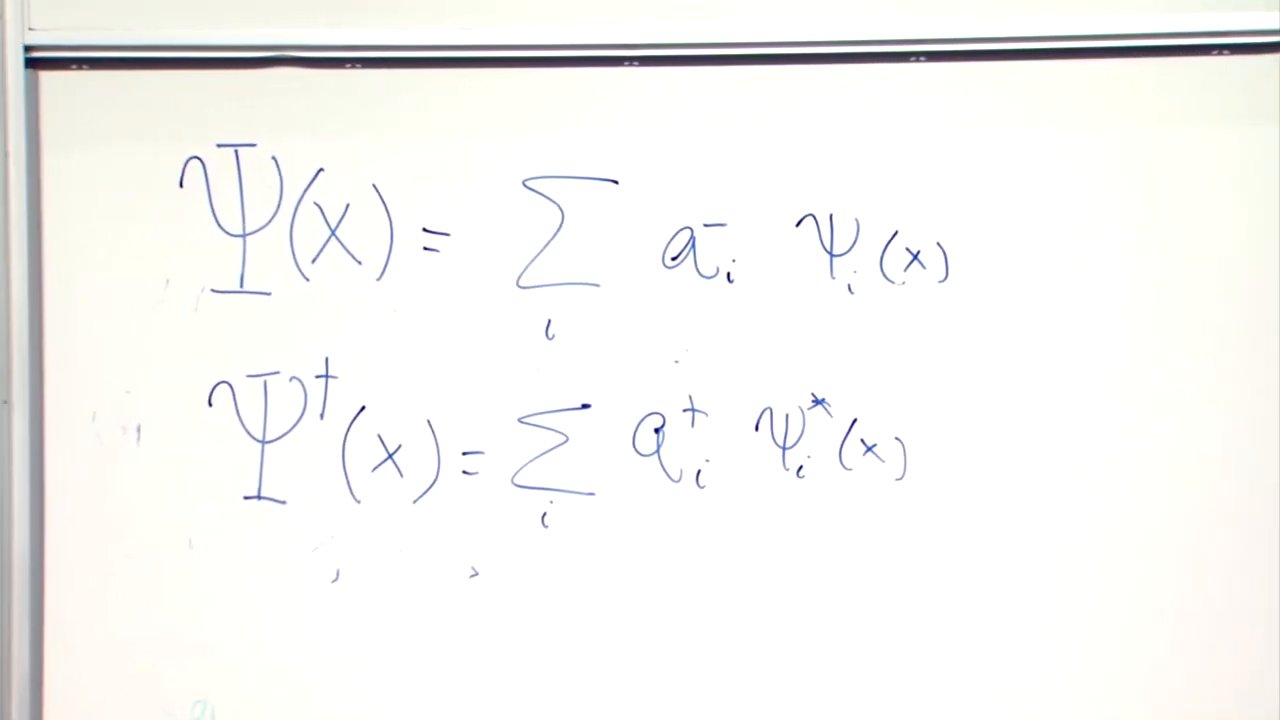
\includegraphics[width=0.9\linewidth]{lecture_06_frame_04.png}
\caption{湮灭场及其厄米共轭的完整模展开。方程~\eqref{eq:l06-field-annihilation}和\eqref{eq:l06-field-creation}在排版形式中保持相同的算符和复共轭结构。}
\lectureframe{01:25:15}
\end{figure}

对于任意固定的位置\(x\)，每个\(\psi_i(x)\)都是普通的复数。所有算符内容都存在于\(a_i\)和\(a_i^\dagger\)中。当\(x\)变化时，我们在空间每一点得到不同的算符。这正是\(\Psi\)是算符值函数的精确含义。

如果基函数是平面波，方程~\eqref{eq:l06-field-annihilation}和\eqref{eq:l06-field-creation}就是量子傅里叶展开：经典傅里叶系数变成了算符。在箱中，基也可以是方程~\eqref{eq:l06-box-basis}中的正弦函数。任何完备正交归一单粒子基都可行。

\(\Psi\)和\(\Psi^\dagger\)都不是厄米的。可观测场可以由厄米组合构成，例如
\begin{equation}
\Psi(x)+\Psi^\dagger(x),
\qquad
i\bigl(\Psi^\dagger(x)-\Psi(x)\bigr),
\end{equation}
而可观测密度稍后将由诸如\(\Psi^\dagger(x)\Psi(x)\)的乘积构成。当前的任务首先是理解这两个基本场做什么。

\begin{classroomqa}
\lecturetimestamp{01:23:14}
\audiencequestion{当右边的模函数是普通波函数时，左边怎么能是算符呢？}
\lecturerresponse{一旦选定\(x\)，函数\(\psi_i(x)\)就是数。因子\(a_i\)是算符。数乘以算符是算符，因此求和也是算符。改变\(x\)就给出整个算符族。}
\end{classroomqa}

\section{场做什么}

湮灭场立即杀死真空：
\begin{equation}
\Psi(x)|0\rangle
=\sum_i\psi_i(x)a_i|0\rangle
=0.
\label{eq:l06-field-kills-vacuum}
\end{equation}
产生场做的事情则信息量大得多。

设\(|i\rangle\)表示波函数为
\begin{equation}
\langle x|i\rangle=\psi_i(x).
\end{equation}
的单粒子态。单粒子基的完备性给出
\begin{equation}
\sum_i|i\rangle\langle i|=1.
\label{eq:l06-completeness}
\end{equation}
将此恒等式作用于一个位置本征态：
\begin{align}
|x\rangle
&=\sum_i|i\rangle\langle i|x\rangle \\
&=\sum_i\psi_i^*(x)|i\rangle.
\label{eq:l06-position-expansion}
\end{align}
在Fock语言中，单粒子模式态为
\begin{equation}
|i\rangle=a_i^\dagger|0\rangle.
\end{equation}
将其代入式~\eqref{eq:l06-position-expansion}，
\begin{align}
|x\rangle
&=\sum_i\psi_i^*(x)a_i^\dagger|0\rangle \\
&=\Psi^\dagger(x)|0\rangle.
\label{eq:l06-local-creation}
\end{align}
因此\(\Psi^\dagger(x)\)产生一个局域在\(x\)处的粒子，而\(\Psi(x)\)则在该处移除一个粒子。位置本征态是{\proseunicodefont δ}函数局域化的，是一个广义的、不可归一化的态；物理上局域化的粒子是通过用可归一化的波包对场进行涂抹而得到的。\editorialnote{本讲采用理想位置本征态的语言。波包这一限定记录了标准的数学含义，而不改变论证。}

\begin{classroomqa}
\lecturetimestamp{01:36:26}
\audiencequestion{指定所产生粒子种类的信息在哪里？\(x\)处的态是{\proseunicodefont δ}函数局域化的吗？}
\lecturerresponse{每一种粒子都被赋予一个单独的场，因此粒子的身份由所使用的场来承载。宗量\(x\)指定了它在何处被产生。在理想位置基中，所产生的态具有{\proseunicodefont δ}函数局域化。}
\end{classroomqa}

玻色子种类的例子包括光子、引力子、希格斯玻色子和胶子，不过现实的场还带有内部指标。即便是光子也需要偏振标签。简化的标量场记号抑制了这些额外的标签，从而使产生原理保持可见。

\subsection{真空不是零矢量}

方程
\begin{equation}
\Psi(x)|0\rangle=0
\end{equation}
包含两个用零表示但非常不同的对象。右矢\(|0\rangle\)是真空：一个归一化的物理态，满足
\begin{equation}
\langle0|0\rangle=1.
\end{equation}
右边的结果是零矢量。它的范数为零；它不能被归一化，也不代表一个物理态。

在加法下这一区别变得鲜明。将零矢量加到一个单粒子态上不改变任何东西。将真空加到一个单粒子态上则给出不同粒子数扇区的真正叠加。在归一化系数下，
\begin{equation}
|\chi\rangle=\frac{1}{\sqrt2}\bigl(|0\rangle+|1\rangle\bigr)
\end{equation}
具有零个粒子和一个粒子的等概率。它不同于\(|1\rangle\)。

\begin{classroomqa}
\lecturetimestamp{01:37:23}
\audiencequestion{如果在\(x\)处没有粒子存在，\(\Psi(x)\)是否就简单地什么都不做？结果为零意味着什么？}
\lecturerresponse{它并不返回原来的态。它返回零矢量。真空是描述空空间的归一化态；零矢量的长度为零，不描述任何物理态。任何算符作用于零矢量都返回零矢量。}
\end{classroomqa}

\begin{classroomqa}
\lecturetimestamp{01:39:00}
\audiencequestion{如果将真空而非零矢量加到一个单粒子态上，会发生什么？}
\lecturerresponse{人们得到一个具有不同粒子数振幅的叠加。相比之下，加上零矢量则使单粒子态保持不变。\(|0\rangle\)中的符号命名的是零占据；它并不意味着零矢量。}
\end{classroomqa}

\begin{classroomqa}
\lecturetimestamp{01:41:56}
\audiencequestion{在场展开式中，模式函数与其产生或湮灭算符的次序重要吗？模式函数是复的吗？}
\lecturerresponse{模式函数是一个普通数，因此与每个算符都对易，所以次序不重要。一般而言模式函数可以是复的；所选基是实的还是复的，取决于单粒子Schr\"odinger问题。}
\end{classroomqa}

\subsection{两个粒子与玻色对称性的出现}

要在\(x\)处产生一个粒子并在\(y\)处产生另一个粒子，作用两次：
\begin{equation}
|x,y\rangle
=\Psi^\dagger(y)\Psi^\dagger(x)|0\rangle.
\label{eq:l06-two-particle-state}
\end{equation}
这两点可以重合也可以不同。由于底层的产生算符对易，
\begin{align}
[\Psi^\dagger(x),\Psi^\dagger(y)]
&=\sum_{i,j}\psi_i^*(x)\psi_j^*(y)
[a_i^\dagger,a_j^\dagger] \\
&=0.
\end{align}
由此可得
\begin{equation}
\Psi^\dagger(y)\Psi^\dagger(x)|0\rangle
=\Psi^\dagger(x)\Psi^\dagger(y)|0\rangle.
\label{eq:l06-boson-exchange}
\end{equation}
交换两个粒子的次序不改变任何东西。这正是玻色交换对称性。因此我们本可以从振子代数出发，\emph{推导出}由对易的产生算符构造出的粒子是玻色子。费米子则需要反对易的算符。

\begin{classroomqa}
\lecturetimestamp{01:42:37}
\audiencequestion{如何将第二个粒子加到单粒子态上？}
\lecturerresponse{作用另一个产生场。要在\(y\)处加上它，就用\(\Psi^\dagger(y)\)作用于\(\Psi^\dagger(x)\)的左侧。结果就是式~\eqref{eq:l06-two-particle-state}中的两粒子态。}
\end{classroomqa}

\begin{classroomqa}
\lecturetimestamp{01:46:04}
\audiencequestion{两个产生场的对易性是否完全等价于将两粒子态对称化？}
\lecturerresponse{是的。它使得一个粒子在\(x\)处、另一个在\(y\)处的态，与交换标签后所得的态完全相同。这正是全同玻色子的定义性交换性质。}
\end{classroomqa}

\begin{classroomqa}
\lecturetimestamp{01:46:32}
\audiencequestion{这是否意味着位于\(x\)和\(y\)处的粒子必须是同一种玻色子？}
\lecturerresponse{是的。自变量\(x\)和\(y\)是位置，而一个场描述一个物种。不同物种，以及诸如两种光子偏振这样的附加标签，需要不同的场分量。}
\end{classroomqa}

\section{为什么可变粒子数很重要}

如果一个问题永远恰好包含三十七个粒子，那么场的语言就只是可选的记账方式。它真正的威力出现在粒子能够被发射和吸收时，尤其是当粒子数本身就是一个量子变量时。Fock空间允许如下形式的态
\begin{equation}
|\Phi\rangle
=c_0|0\rangle+c_1|1\rangle+c_2|2\rangle+\cdots,
\qquad
\sum_{n=0}^{\infty}|c_n|^2=1.
\end{equation}
激光场是一个重要的例子：它一般并不是具有一个确定光子数的态，而是许多数扇区的叠加。

粒子与场之间的桥梁现在已明确建立。模式算符对能量本征态中的粒子进行计数并改变粒子数；场将这些算符与一组完备的波函数结合起来，从而可以在指定位置产生或移除粒子。谐振子的代数已成为玻色子量子场的基本语言。
